\chapter{Estado del Arte}

De los trabajos que existen en la actualidad, podemos mencionar tres que resultan de especial interés para este trabajo de investigación. Las tres metodologías de nuestro interés son las siguientes:
\begin{itemize}
	\item Búsqueda de reglas locales para un autómata celular mediante el análisis estadístico de las observaciones de un fenómeno.
	\item Configuración de reglas locales para un autómata celular mediante el empleo de algoritmos evolutivos.
	\item Búsqueda de reglas locales para un autómata celular mediante el empleo de algoritmos evolutivos para satisfacer un patrón específico.
\end{itemize}

Estos son algunos de los enfoques para emplear los autómatas celulares como herramienta para modelar fenómenos, que si bien tienen relación con este trabajo de tesis en el aspecto de buscar configurar o encontrar reglas de evolución para un autómata celular, no se conectan directamente con él debido a que emplean otros enfoques como las tres metodologías que se mencionaron previamente.

\section{Análisis estadístico para el descubrimiento de reglas }

Uno de los enfoques como se ve en \citep{kawaharada2016cellular}, se centra en descubrir reglas de evolución para un autómata celular unidimensional, empleando métodos de análisis estadísticos para determinar dichas reglas, a partir de los datos observados de los patrones de bioconvección que son generados como resultado de la respuesta a la estimulación luminosa de un tipo de alga unicelular llamada \emph{Euglena gracilis}.
\\

El experimento consistió en iluminar por la parte de abajo de un contenedor anular conteniendo una suspensión de E. gracilis con una fuerte intensidad de luz. Los individuos, al ser alcanzados por la luz, sufren de fototaxis negativa, lo cual provoca que se acumulen cerca de la superficie.
\\

Como la densidad del E. gracilis es mas pesada que el agua, las regiones ricas en esta alga se precipitan al fondo para conducir el flujo local. Estas interacciones entre los individuos y el flujo eventualmente forma patrones de bioconvección.
\\

El proceso se realizó de la siguiente forma:

\begin{enumerate}
	\item Recopilación de imágenes de los patrones de bioconvección.
	\item Transformación de las imágenes recopiladas a escala de grises.
	\item Uso de filtros para la eliminación del ruido.
	\item Discretización de las imágenes en escala de grises.
	\item Se predetermina el número de estados para el sitio $k$ y se discretiza la información observada acorde a esto.
	\item Basado en el número de vecinos establecido $m$ se calcula la frecuencia con la que aparecen los estados por cada combinación de posibles estados vecinos.
	\item Con base en esta frecuencia se determinan las reglas locales para el Autómata Celular (AC).
\end{enumerate}


Como se puede observar en los pasos \emph{6} y \emph{7} del proceso anterior, la determinación de las reglas locales del AC se realiza por medio de la frecuencia en la que aparecen los estados y resulta en reglas locales especializadas que definen su comportamiento; además, es importante mencionar que éste comportamiento está establecido de acuerdo a los datos que se utilizaron para obtener las reglas.


El algoritmo que se propone en este trabajo de tesis logra realizar una búsqueda más robusta en el espacio de reglas, para obtener un conjunto de reglas con un comportamiento generalizado que se encuentra establecido en los datos.

\section{Configuración de reglas para un AC con algoritmos evolutivos}

En \cite{naghibi2016discovery} se muestra un método para descubrir las reglas de transición de un autómata celular de lattice bidimensional que modele el crecimiento urbano empleando un algoritmo de optimización de colonia de abejas artificiales. Para ello, se utilizan como datos de entrada información multitemporal sensada remotamente de el área urbana de la ciudad de Urmia, Irán.
\\

El autómata celular en este trabajo se define con la siguiente ecuación:

\begin{equation} \label{eq:8}
P^t_{ij} = S^t_{ij}\times\Omega^t_{ij}\times Con\times e_r,
\end{equation}

donde:
\begin{itemize}
	\item $P^t_{ij} $ es el potencial de desarrollo de una celda $ij$.
	\item $S^t_{ij}$ es la idoneidad de la celda $ij$ para cambiar basada en factores relevantes en el tiempo $t$.
	\item $\Omega^t_{ij}$ es el efecto que tiene la densidad de desarrollo del vecindario.
	\item $Con$ es una condición funcional que se vuelve verdadero cuando se encuentra la idoneidad de la celda.
	\item $e_r$ es un término para la perturbación estocástica por errores.
\end{itemize}

El potencial de desarrollo se compara con un valor umbral para determinar si una célula no urbanizada va a poder ser transformada en una célula urbanizada en el tiempo $t+1$. Entonces, los valores a encontrar son los valores de umbral para los cuales se produce la transición de una célula no urbanizada a una urbanizada.
\\

Como requerimiento para la evaluación del algoritmo, se emplean otras dos técnicas además de la colonia de abejas artificiales, las cuales son:
\begin{itemize}
	\item Particle Swarm Optimization (PSO)
	\item Logistic Regression
\end{itemize}

La figura \ref{fig:abc} muestra el procedimiento que se siguió para la calibración de las reglas del autómata celular, utilizando un algoritmo de optimización de colonia de abejas artificiales.

\begin{figure}[H]
	\centering
	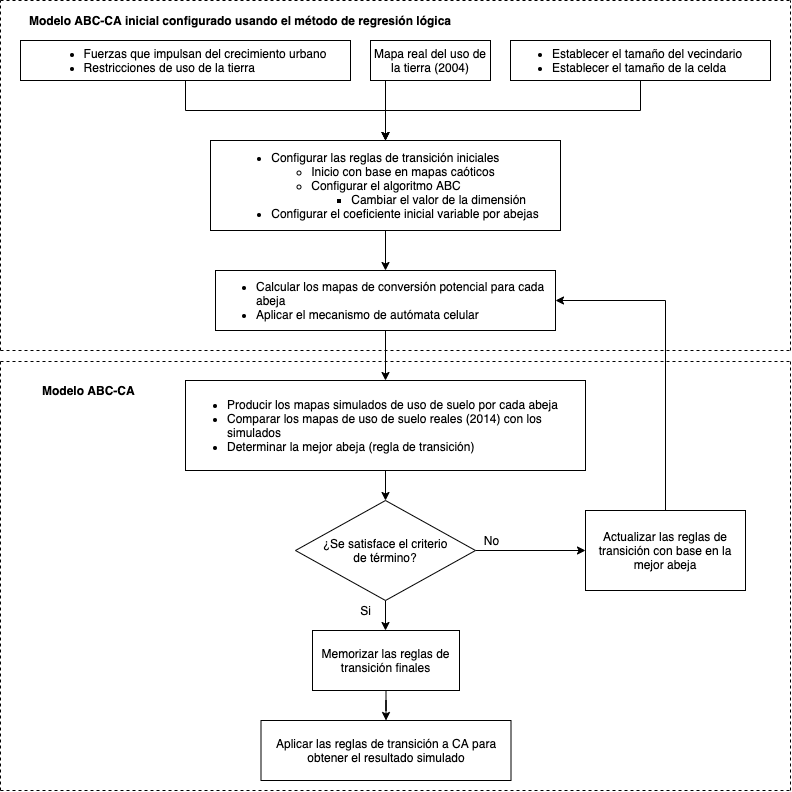
\includegraphics[width=\linewidth]{fig/abejas}
	\caption{Modelo para la obtención de reglas del autómata celular empleando un algoritmo de optimización de colonia de abejas artificiales. Diagrama traducido de \cite{naghibi2016discovery}.}
	\label{fig:abc}
\end{figure}

Como vemos en la figura \ref{fig:pso} y en la figura \ref{fig:abc}, son similares los procesos si no tomamos en cuenta las particularidades de cada algoritmo, un proceso de simulación, uno de evaluación, y por ultimo un proceso de actualización, son las partes que identifican un proceso general de aprendizaje.

\begin{figure}[H]
	\centering
	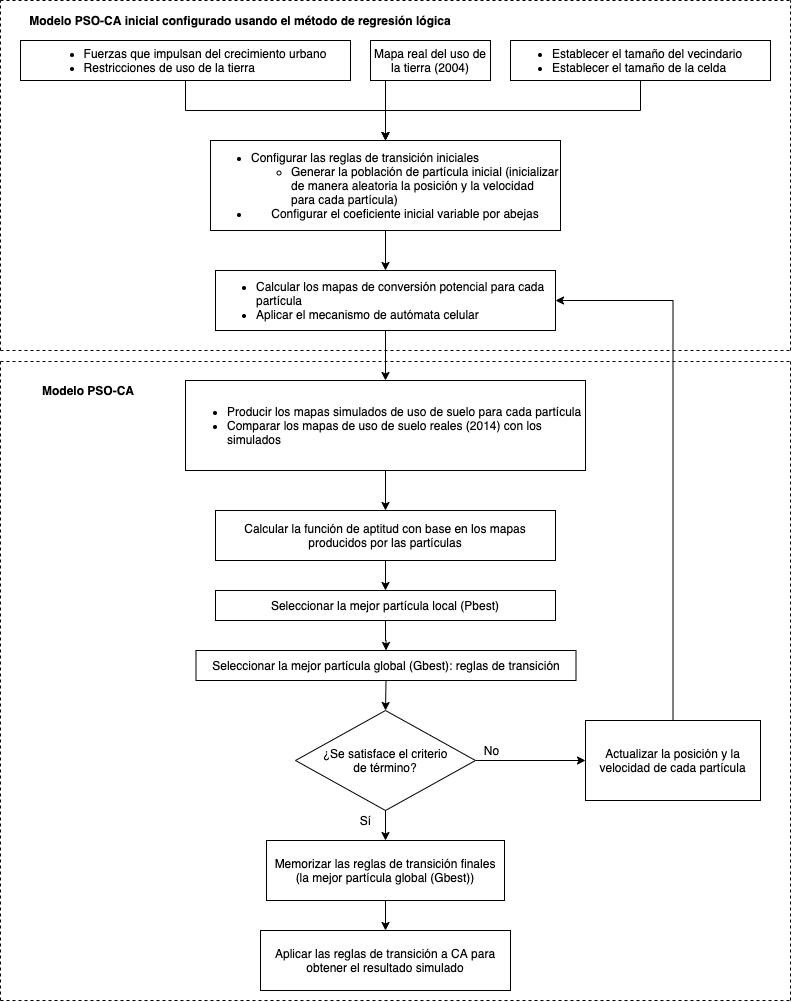
\includegraphics[width=\linewidth]{fig/particulas}
	\caption{Modelo para la obtención de reglas del autómata celular empleando un algoritmo de optimización de enjambre de partículas. Diagrama traducido de \cite{naghibi2016discovery}.}
	\label{fig:pso}
\end{figure}

En la figura \ref{fig:evaluation} vemos el proceso que se siguió para realizar la evaluación de los 3 algoritmos, simulando cada uno por separado, después comparando el resultado de la simulación con la realidad y entonces obteniendo el porcentaje de exactitud de la simulación.

\begin{figure}
	\centering
	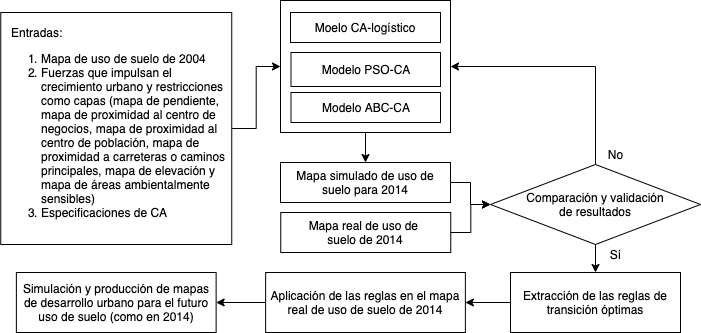
\includegraphics[width=\linewidth]{fig/evaluacion}
	\caption{Modelo de evaluación de los algoritmos. Diagrama traducido de \cite{naghibi2016discovery}.}
	\label{fig:evaluation}
\end{figure}
\renewcommand{\arraystretch}{1.5}
\begin{table}[H]
	\begin{center}
		\begin{tabular}{p{5.8cm} c c c}
		\hline
		\multirow{2}{0.5\linewidth}{\textbf{\small Validation Method}} & \multicolumn{3}{c }{\textbf{\small Prediction Approach}}\\
		\cline{2-4}
		&\textbf{\small CA-Logistic}&\textbf{\small PSO-CA}&\textbf{\small ABC-CA}\\
		\hline
		{\small Overall accuracy (\%)}&{\small 82.8}&{\small 87.5}&{\small  89} \\
		\hline
		{\small Figure of merit (\%)}&{\small 30}&{\small 32.6}&{\small 35.7 } \\
		\hline
\end{tabular}
\end{center}
\end{table}
\begin{table}[H]
	\begin{center}
		\begin{tabular}{p{5.8cm} c c c}
		{\small False alarms (\%)}&{\small 15.1}&{\small 7.7}&{\small 6.2 } \\
		\hline
		{\small Misses (\%)}&{\small 2.1}&{\small 4.8}&{\small 4.8 } \\
		\hline
		{\small Allocation disagreement (\%)}&{\small 17.2}&{\small 12.5}&{\small 11 } \\
		\hline
		{\small Correctly predicted unchanged cells (\%)}&{\small 75.4}&{\small 81.4}&{\small 82.9 } \\
		\hline
		{\small Protection of agricultural areas from urbanization (\%)}&{\small 62.2}&{\small 68.6}&{\small 74.1 } \\
		\hline
		{\small Areas of the simulated gain of the urban lands in 2004-2014 (the actual gain area of the city is 2500 hectares) (hectares)}&{\small 4960}&{\small 3155}&{\small 2824 } \\
		\hline
		{\small TOC (closeness to maximum boundary)}&{\small low}&{\small medium}&{\small high } \\
		\hline
		\end{tabular}
	\end{center}
	\caption{Resultados de la evaluación de los algoritmos. Tabla obtenida de \cite{naghibi2016discovery}. }
	\label{fig:results}
\end{table}

Como podemos ver en la tabla de resultados \ref{fig:results}, el algoritmo de colonia de abejas fue capaz de obtener un mejor rendimiento en comparación con los otros métodos. Esto ayudará a obtener un mejor despeño en la estimación correcta del crecimiento urbano. Sin embargo, el método aquí planteado sigue teniendo ciertos obstáculos como lo es encontrar una correcta definición de la ecuación que determine al autómata celular, por ejemplo la ecuación \ref{eq:8} que se usa en este trabajo. 


\section{Búsqueda de reglas de evolución para replicar estructuras}

El aporte principal de \cite{bidlo2016routine} es la creación de un método para la obtención de un conjunto de reglas que puedan replicar un comportamiento específico. Sin embargo, es importante resaltar que no se toma en cuenta conocimiento previo del fenómeno que se quiere replicar. Lo que se utiliza es un algoritmo evolutivo, cuya función de aptitud es dependiente del resultado al que se quiere llegar. La codificación de las reglas viene dada de la siguiente forma:

\begin{figure}[H]
	\centering
	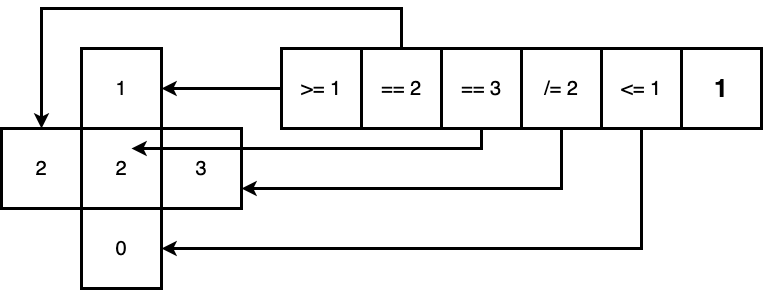
\includegraphics[width=\linewidth]{fig/codreglas}
	\caption{Ejemplo de la codificación de las reglas de evolución del autómata con un vecindario de tipo Moore. Figura obtenida de \cite{bidlo2016routine}.}
	\label{fig:rulesencoding}
\end{figure}

De este artículo \citep{bidlo2016routine} encontramos especialmente útil la forma en que se codificaron las reglas, esto sirvió como inspiración, para el diseño de la representación de las reglas en el algoritmo propuesto en este trabajo.

\nomenclature{AC}{Autómata Celular}
\nomenclature{PSO}{Particle Swarm Optimization}
\nomenclature{ABC}{Artificial Bees Colony}